\documentclass[aspectratio=169]{beamer}

\usepackage[backend=bibtex]{biblatex}
\bibliography{../thesis/references}
%\bibliographystyle{ieeetr}
%
% Choose how your presentation looks.
%
% For more themes, color themes and font themes, see:
% http://deic.uab.es/~iblanes/beamer_gallery/index_by_theme.html
%
\mode<presentation>
{
  \usetheme{default}      % or try Darmstadt, Madrid, Warsaw, ...
  \usecolortheme{default} % or try albatross, beaver, crane, ...
  \usefonttheme{default}  % or try serif, structurebold, ...
  \setbeamertemplate{navigation symbols}{}
  \setbeamertemplate{caption}[numbered]
} 

\usepackage[english]{babel}
\usepackage[utf8]{inputenc}
\usepackage[font=small]{caption}
\usepackage[absolute,overlay]{textpos}
\usepackage{graphicx}
\usepackage{hyperref}
\usepackage{animate}
\graphicspath{ {../thesis/img/} }

\title[Consensus Clustering]{Tool for Visual Cluster Analysis and Consensus Clustering}
\author{Christian Permann}
\institute{Faculty of Computer Science, University of Vienna,\newline W\"ahringer Stra{\ss}e 29, 1090 Vienna}
\date{TBD.04.2020}

\begin{document}

\begin{frame}
  \titlepage
\end{frame}

% Uncomment these lines for an automatically generated outline.
%\begin{frame}{Outline}
%  \tableofcontents
%\end{frame}

\begin{frame}{Introduction}
	Clustering:
	\begin{itemize}
		\item Grouping data-points such that their underlying relationships are reflected
		\item Gaining knowledge through this grouping
	\end{itemize}

	\begin{center}
		The process of clustering is not done when a solution is computed,\newline but when the researcher involved:\newline
		``... \textbf{evaluated}, \textbf{understood} and \textbf{accepted} the patterns.'' (Chen and Liu \cite{VISTA})
	\end{center}
	
	Challenges:
	\begin{itemize}
		\item Many possibilities for clustering:
		\begin{itemize}
			\item Algorithms/Parameters/Assumptions
		\end{itemize}
		\item Choice and interpretation of solution is difficult
	\end{itemize}

\end{frame}



\begin{frame}{Related Work: Clustering}
	There is a vast amount of clustering techniques, including:\newline
	\begin{itemize}
		\item Partition-based methods (KMeans-like algorithms)
		\item Hierarchy-based methods (e.g. Joining of Sets/Linking)
		\item Density-based methods (e.g. DBSCAN/OPTICS)
		\begin{itemize}
			\item Many more...
		\end{itemize}
	\end{itemize}
\end{frame}

\begin{frame}{Related Work: Visual Frameworks}
	\begin{itemize}
		\item ClusterVision
		\begin{itemize}
			\item Ranking solutions according to a combination of quality metrics
			\item Choosing from the highest ranked ones
		\end{itemize}
		\item VISTA		
		\begin{itemize}
			\item In-depth analysis of individual solutions
			\item Possibilities for relabeling of points (ClusterMap)
		\end{itemize}
		\item Simple Visualizations
		\begin{itemize}
			\item Included in most data-analysis tools
			\item Scatter plots, bar charts, etc.
		\end{itemize}
	\end{itemize}
\end{frame}

\begin{frame}{Related Work: Consensus Clustering}
	Combining clustering results may yield a better solution:
	\begin{figure}
	  \centering
	    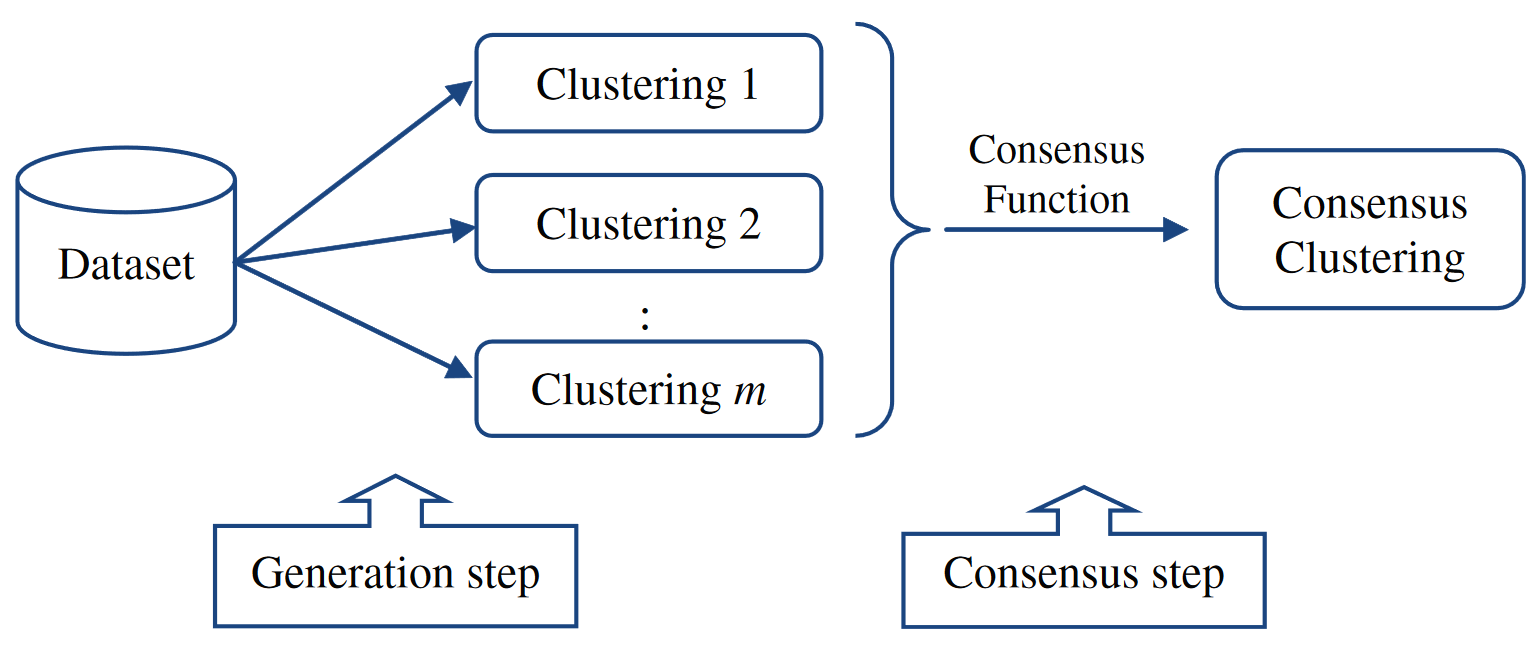
\includegraphics[width=0.6\textwidth]{flow}
	  \caption{Workflow for generating consensus clusterings \cite[p.~340]{survey1}}
	  \label{fig:flow}
	\end{figure}
\end{frame}



\begin{frame}{Idea of our Tool: Facilitating clustering exploration}
How can we assist users in exploring clustering results?\newline
	\begin{itemize}
		\item Visualizing individual results
		\begin{itemize}
			\item Scatter plot (matrices)/kernel density estimation
			\item Dimensionality reduction
		\end{itemize}
		\item Visualizing similarities between results
		\begin{itemize}
			\item OPTICS meta-clustering
			\item Heat maps
			\item Multi-Dimensional-Scaling to approximate solution space
		\end{itemize}
	\end{itemize}
\end{frame}

\begin{frame}{Idea of our Tool: Gathering more Information}
Can we gain additional knowledge from multiple computed solutions?\newline
	\begin{itemize}
		\item Previous frameworks only try to select the best one
		\begin{itemize}
			\item Additional information lost
			\item Difficult to objectively identify best one
		\end{itemize}
		\item Consensus clustering
		\begin{itemize}
			\item Can combine solutions or groups of solutions
		\end{itemize}
	\end{itemize}

Idea:
	\begin{itemize}
		\item Combine group of robust solutions into one
	\end{itemize}
\end{frame}

\begin{frame}{The Tool}
	
	Three main parts:
	\begin{itemize}
		\item Data-View
		\begin{itemize}
			\item Loading/Saving/Creating data
			\item Cleaning up data
			\item Visualizing data
		\end{itemize}
		\item Workflow-View
		\begin{itemize}
			\item Creating clustering workflows
			\item Defining parameters
		\end{itemize}
		\item Meta-View
		\begin{itemize}
			\item Visualizing clusterings and meta-clusterings
			\item Selecting or creating final results (\& consensus clustering)
		\end{itemize}
	\end{itemize}

\end{frame}

\begin{frame}{The Tool: Data-View}
	
	\begin{figure}
	  \centering
	    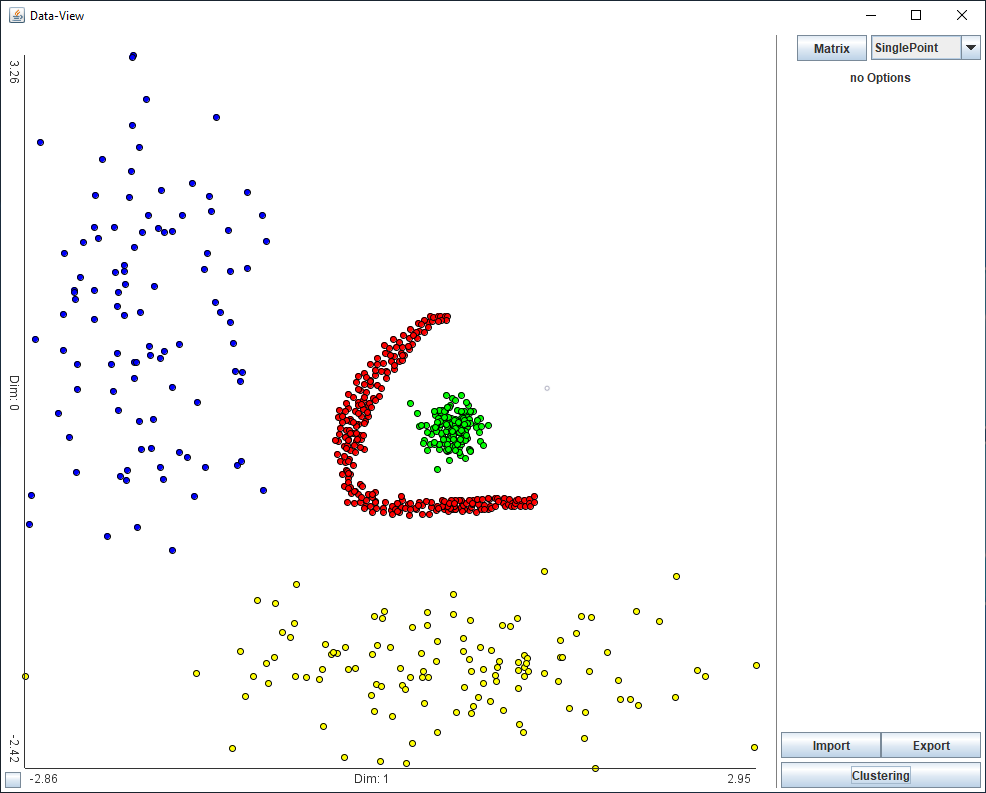
\includegraphics[width=.64\textwidth]{unob}
	  \caption{Data-View}
	  \label{fig:data-view}
	\end{figure}

\end{frame}

\begin{frame}{The Tool: Data-View - Scatter Plot Matrix}
	
	\begin{figure}
	  \centering
	    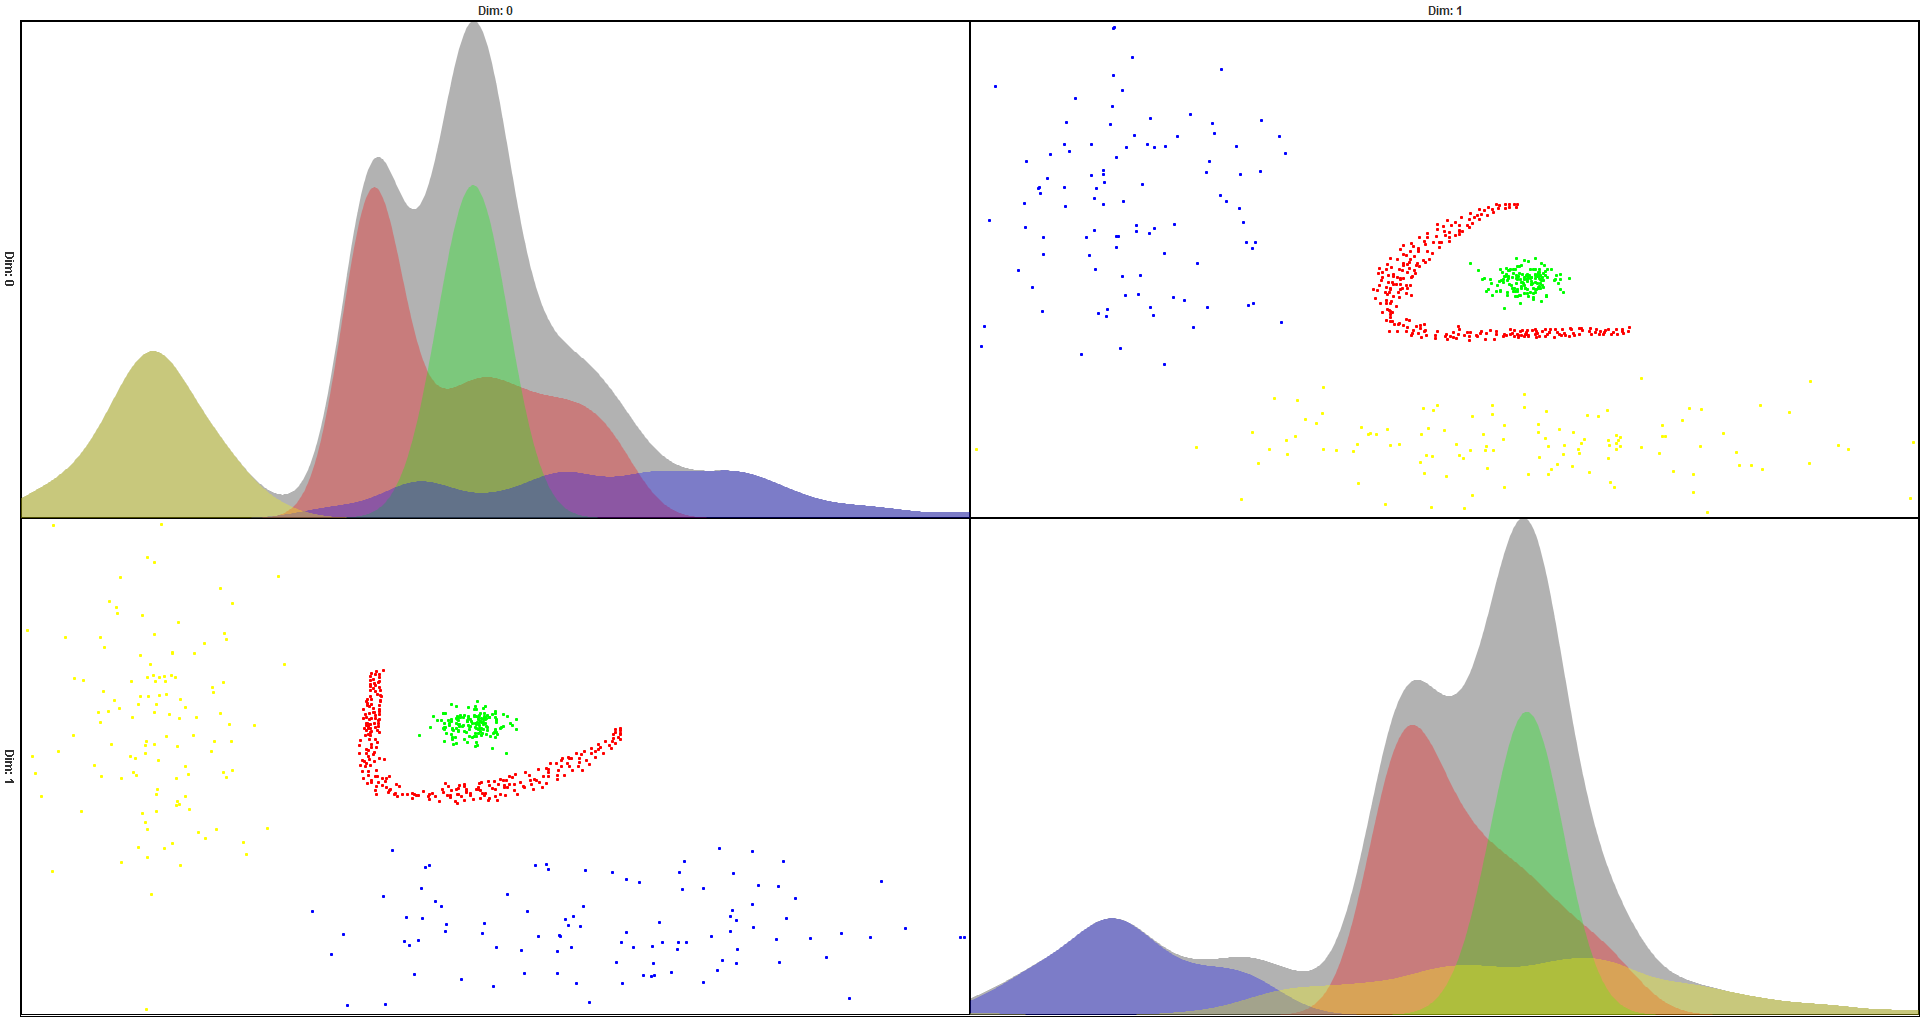
\includegraphics[width=.97\textwidth]{scatter_matrix}
	  \caption{Scatter Plot Matrix}
	  \label{fig:scatter_matrix}
	\end{figure}

\end{frame}

\begin{frame}{The Tool: Workflow-View}
	
	\begin{figure}
	  \centering
	    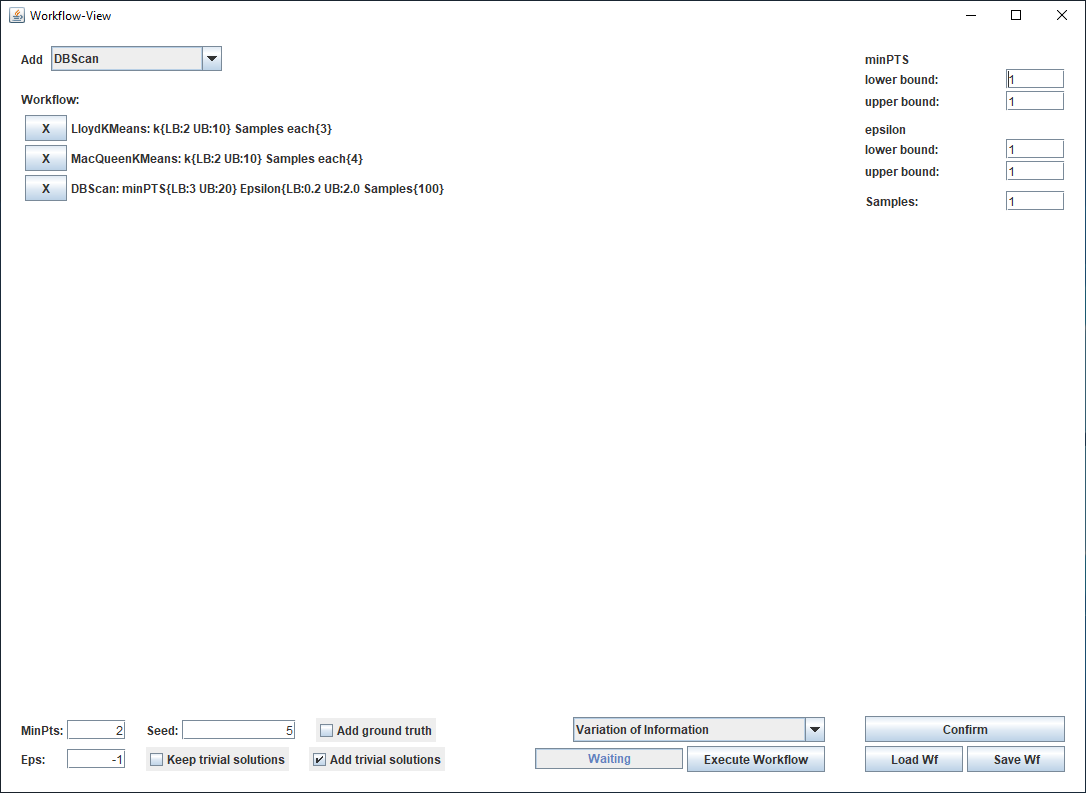
\includegraphics[width=.7\textwidth]{workflow-view-tasks}
	  \caption{Workflow-View}
	  \label{fig:workflow-view}
	\end{figure}

\end{frame}

\begin{frame}{The Tool: Meta-View}
	
	\begin{figure}
	  \centering
	    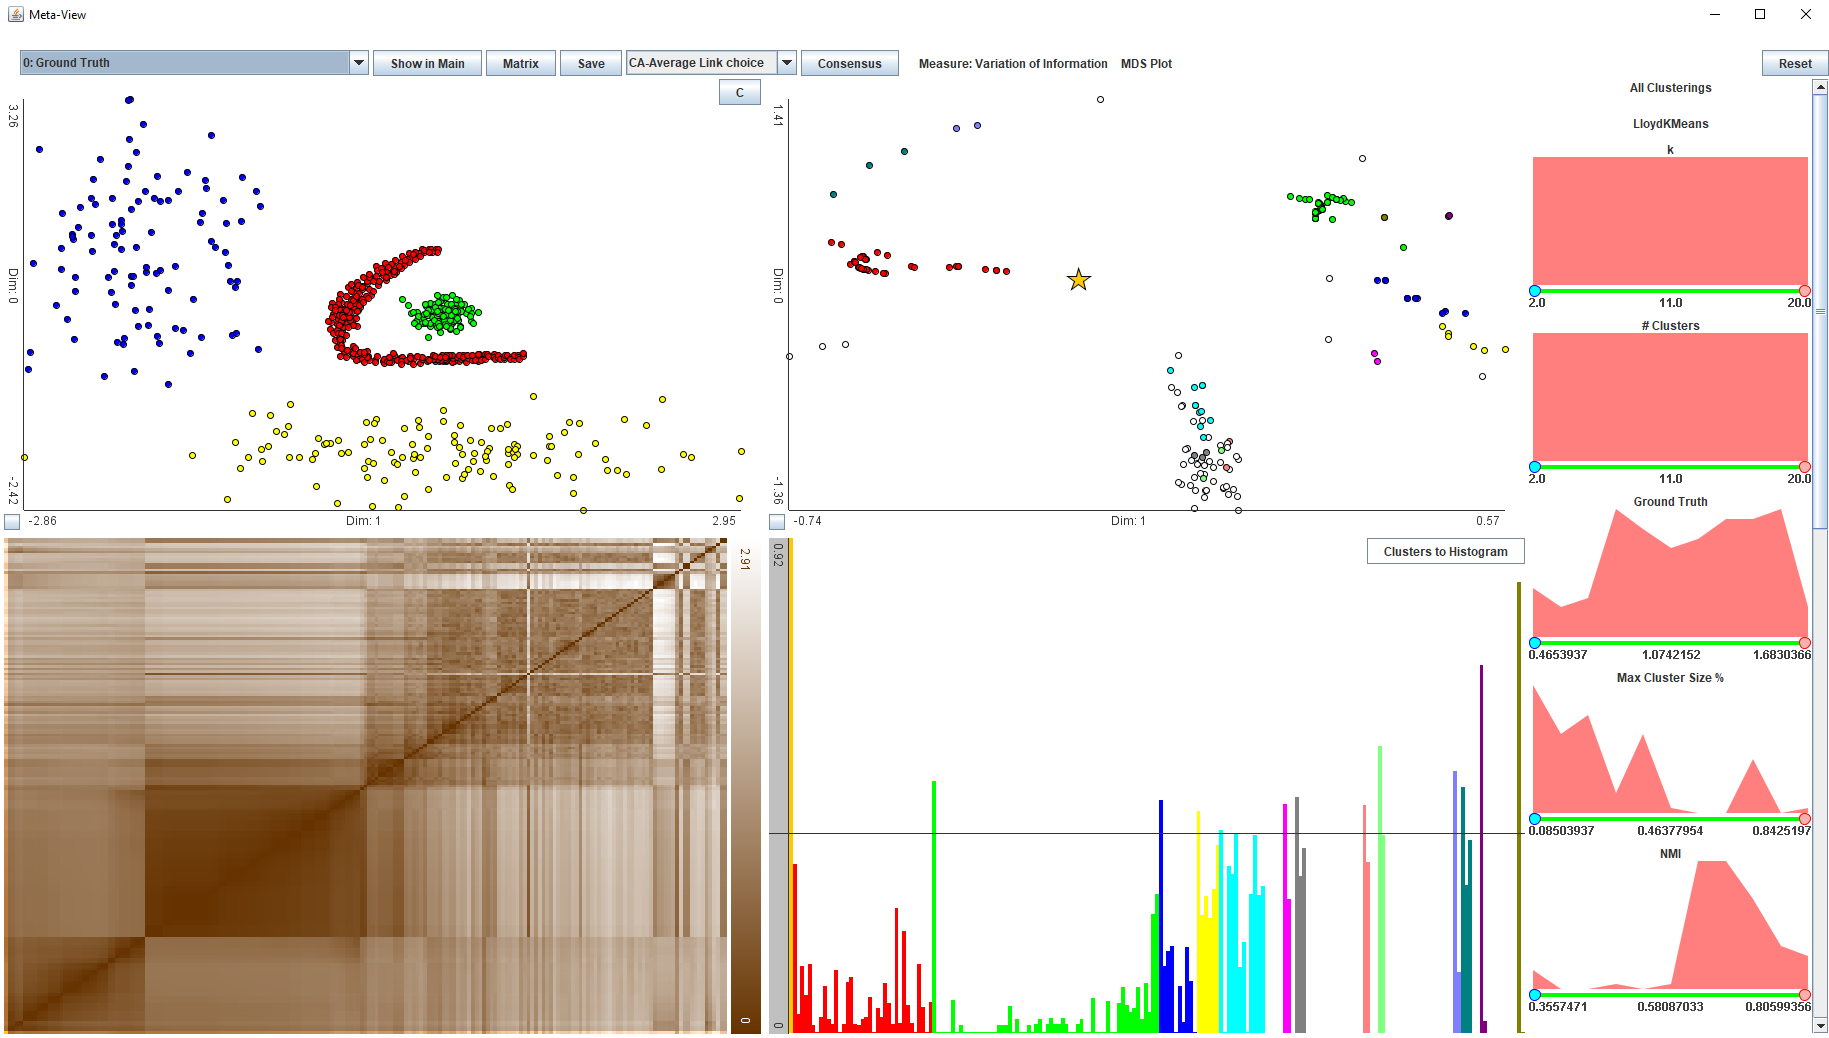
\includegraphics[width=.9\textwidth]{meta-view}
	  \caption{Meta-View}
	  \label{fig:meta-view}
	\end{figure}

\end{frame}


\begin{frame}{Implementation}
Used tools:
	\begin{itemize}
		\item Java 1.8, utilizing Streams for parallelization
		\item Libraries:
		\begin{itemize}
			\item  ELKI \cite{10.1007/978-3-540-69497-7_41} - Clustering
			\item WEKA \cite{10.1145/1656274.1656278} - IO
			\item Java Smile \cite{javasmile} - Additional Methods
		\end{itemize}
		\item Swing's JComponents and overriding the \emph{draw()} method
		\item[]
	\end{itemize}
Ease of extension:
	\begin{itemize}
		\item All selectable methods provide simple interfaces
	\end{itemize}
\end{frame}


\begin{frame}{Tests}
	
	\begin{itemize}
		\item bla
	\end{itemize}

\end{frame}


\begin{frame}{Future Work}

	\begin{itemize}
	 	\item bla
	\end{itemize}

\end{frame}


\begin{frame}{Conclusion}

	\begin{itemize}
		\item bla
		\item[]
		\item Link to the tool:
		\begin{itemize}
			\item \url{https://github.com/chris9182/Visual_Cluster_Exploration}
		\end{itemize}
	\end{itemize}

\end{frame}

\begin{frame}[allowframebreaks]{References}
\printbibliography
\end{frame}

\end{document}